\pagestyle{myheadings}
\markboth{BÖLÜM 1. GİRİŞ}{1.1. DİL İŞLEMCİLERİ}
\renewcommand{\chaptername}{Bölüm}

\chapter{Giriş}
Programlama dilleri, hesaplamaları insanlar ve bilgisayarlar için tanımlayan notasyonlardır. İçinde bulunduğumuz dünya programlama dillerine bağımlıdır, çünkü var olan tüm bilgisayarlar üzerinde çalışan tüm yazılımlar bir programlama dili ile yazıldı. Fakat, bir program çalışmaya başlamadan önce bilgisayarın onu anlayacağı bir forma çevrilmelidir.

Bu çevrimi yapan yazılım sistemlerine  \textit{derleyici} denir.

Bu kitap derleyicilerin nasıl tasarlanıp uygulanacakları hakkındadır. Burada dönüştürücülerin birkaç temel fikir kullanılarak geniş çeşitlilikte diller ve makineler için oluşturulabileceğini keşfedeceğiz. Derleyicilerin yanı sıra, derleyici tasarımında kullanılan prensip ve teknikler o kadar çok alanda uygulanabilirdir ki, yüksek ihtimalle bir bilgisayar bilimcisinin/mühendisinin kariyerinin bir çok noktasında tekrar tekrar kullanılacaktır. Derleyici yazımı'nın çalışılması, programlama dilleri, makine mimarileri, dil teorisi, algoritmalar ve yazılım mühendisliği olmak üzere bir çok noktaya dokunur.

Bu ilk bölümde, dil dönüştürücülerin değişik formlarını, tipik bir derleyicinin yapısını kabaca gözden geçirecek ve derleyicileri şekillendiren programlama dilleri ve bilgisayar mimarileri trendlerinden bahsedeceğiz. Ayrıca bilgisayar bilimi ve derleyici tasarımı teorisi arasındaki ilişki ve derlemenin de ötesine geçen derleyici teknolojilerinin genel hatları üzerine gözlemleri de işleyeceğiz. Son olarak derleyici çalışmamız için gerekli olan anahtar programlama-dili konseptleri'ni özetleyerek bitireceğiz.

\section{Dil İşlemcileri}

Basitçe, derleyici, bir dilde yazılmış -\textit{kaynak} dil- herhangi bir programı okuyup başka bir dile -\textit{hedef} dil -  eşdeğer olarak çeviren bir programdır; bkz. Şekil 1.1. Derleyicinin önemli bir rölü, dönüşüm sırasında kaynak dilde tespit ettiği hataları bildirmesidir.

\begin{center}
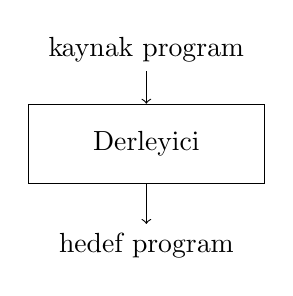
\begin{tikzpicture}[->]

\tikzstyle{rect} = [rectangle, minimum width=3cm, minimum height=1cm,text centered, draw=black]
\node (src)  {kaynak program};
\node (tr) [below of=src, yshift=-1.5cm] {hedef program};
\node (dr) [rect, below of=src, yshift=-0.2cm] {Derleyici};   
   
\draw [black](src) -- (dr);  
\draw [black](dr) -- (tr);  

\end{tikzpicture}

Şekil 1.1: Bir derleyici
\end{center}



Eğer hedef program çalıştırılabilir bir makine-dili programıysa, kullanıcı tarafından girdileri işlemesi ve çıktı üretmesi için kullanılabilir; bkz. Şekil 1.2.

\begin{center}
\begin{tikzpicture}[->]

\tikzstyle{rect} = [rectangle, minimum width=3cm, minimum height=1.5cm,text centered, draw=black]

\node (in) [left of=src, xshift=-1.5cm] {girdi};
\node (out)[right of=src, xshift=1.5cm]   {çıktı};
\node (tr) [rect] {Hedef Program};   
   
\draw [black](in) -- (tr);  
\draw [black](tr) -- (out);  

\end{tikzpicture}

Şekil 1.2: Hedef Programı Çalıştırmak

\end{center}

\renewcommand{\thefootnote}{\fnsymbol{footnote}}
\textit{Yorumlayıcı\footnote{(İng.) Interpreter. (Ç.N.)}} da yaygın bir dil işlemci tipidir. Şekil 1.3'te görüldüğü gibi hedef programını üretirken bunu çevrim olarak yapmaktansa, yorumlayıcı, kaynak programın içindeki komutları direkt olarak, kullanıcı tarafından sağlanan girdiler üzerinden çalıştırır.

\begin{center}
\begin{tikzpicture}[->]

\tikzstyle{rect} = [rectangle, minimum width=3cm, minimum height=1.5cm,text centered, draw=black]

\node (in) [left of=src, xshift=-1.5cm, yshift=-0.3cm] {girdi};
\node (src) [left of=src, xshift=-3cm, yshift=0.4cm] {kaynak program};
\node (out)[right of=src, xshift=6cm,yshift=-0.4cm]   {çıktı};
\node (tr) [rect] {Yorumlayıcı};   
   
\draw [black](in) -- (tr.192);  
\draw [black](src) -- (tr.165);  
\draw [black](tr) -- (out);  

\end{tikzpicture}

Şekil 1.3: Hedef Programı Çalıştırmak
\end{center}


Girdileri çıktılara eşleyen bir yorumlayıcıdansa, derleyici tarafından üretilmiş bir makine-dili hedef programı genellikle daha hızlıdır. Bununla beraber, bir yorumlayıcı, hataları genellikle bir derleyiciden daha iyi teşhis edebilir, çünkü yorumlayıcı kaynak programı satır satır çalıştırır.

\paragraph{Örnek 1.1:}
Şekil 1.4'te görüldüğü gibi Java dil işlemcileri derlemeyi ve yorumlamayı beraber kullanır. Java kaynak programı önce \textit{bytecode} denilen bir ara form'a çevrilir. Ardından bytecode'lar bir sanal makine tarafından yorumlanır. Bu tür bir ayarlamanın avantajı, bir makinede derlenen bir kodun başka bir makinede ya da bir ağ üzerindeki makinelerde yorumlanabilmesidir.

Girdilerin çıktılara dönüştürülmesini hızlandırmak için, \textit{tam-zamanında} derleyiciler denilen bazı Java derleyicileri, bytecode'ları ara program girdileri işlemeden önce,  anlık olarak makine diline çevirir. 

\begin{center}
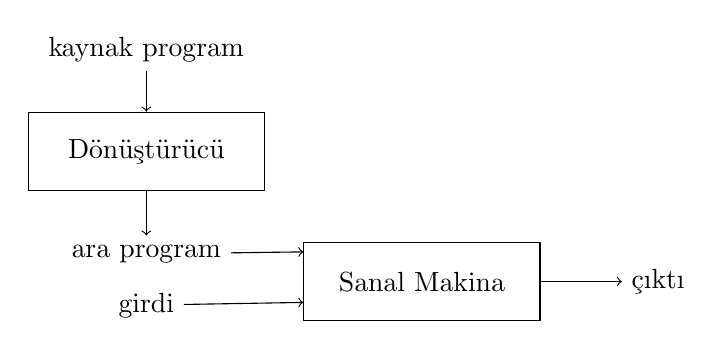
\begin{tikzpicture}[->]

\tikzstyle{rect} = [rectangle, minimum width=3cm, minimum height=1cm,text centered, draw=black]

\node (src_p)   {kaynak program};
\node (translator) [rect, below of=src_p, yshift=-0.3cm] {Dönüştürücü};   
\node (intermediate_p) [below of=translator, yshift=-0.3cm] {ara program};
\node (in) [below of=intermediate_p, yshift=0.35cm] {girdi};
\node (vm) [rect, right of=in, xshift=2.5cm, yshift=0.3cm, ] {Sanal Makina};   
\node (out) [right of=vm,xshift=2cm] {çıktı};

\draw [black](src_p) -- (translator);  
\draw [black](translator) -- (intermediate_p);  
\draw [black](intermediate_p) -- (vm.166);  
\draw [black](in) -- (vm.190);  
\draw [black](vm) -- (out);  

\end{tikzpicture}

Şekil 1.4: Bir hibrid derleyici
\end{center}

Şekil 1.5'te gösterildiği gibi bir derleyiciye ek olarak, çalıştırılabilir bir hedef program oluşturmak için birkaç program daha gerekli olabilir. Bir kaynak program ayrı dosyalarda tutulan modüllerden oluşmuş olabilir. Bu kaynak kodu toparlamak bazen \textit{önişlemci} denlilen başka programlara havale edilir. Önişlemci ayrıca makro denilen kısayolları kaynak kodun ifadelerine çevirebilir.

Ardından düzenlenmiş kaynak kodu derleyiciye yüklenir. Derleyici çıktısı olarak assembly-dili programı üretebilir, çünkü assembly üretimi ve hata ayıklaması kolay bir programdır. Ardından assembly dili, yeniden konumlandırılabilir makine kodu üreten ve \textit{assembler} denilen bir programda işlenir.

Büyük programlar genelde parçalar halinde derlenir, böylece yeniden konumlandırılabilir makina kodu, makinada çalışan diğer yeniden konumlandırılabilir nesne ve kütüphane dosyaları ile bağlanabilir. \textit{Bağlayıcı} bir dosyadaki dosyanın başka bi dosyadaki dosyaya ulaşması için harici hafıza adreslerini çözümler. \textit{Yükleyici} sonra tüm bu çalıştırılabilir nesne dosyalarını bir araya getirip çalıştırılmak üzere hafızaya yükler.  

\subsection{Bölüm 1.1 için Alıştırmalar}

\paragraph{Örnek 1.1.1:} Bir yorumlayıcı ile derleyicinin arasındaki fark nedir?

\paragraph{Örnek 1.1.2:}  a ve b maddelerin avantajları nelerdir?; a) Bir yorumlayıcı üzerine bir derleyici. b) Bir derleyici üzerine bir yorumlayıcı.

\paragraph{Örnek 1.1.3:} Derleyicinin makina dilindense assembly dili ürettiği bir dil-işleme sisteminin avantajları nelerdir?

\paragraph{Örnek 1.1.4:} Yüksek seviyeli bir dili başka yüksek seviyeli bir dile çeviren derleyiciye \textit{kaynaktan-kaynağa} dönüştürücü denir. C dilini bir derleyici için kaynak dil olarak kullanmanın avantajları ne olur?

\setcounter{footnote}{0}
\paragraph{Örnek 1.1.5:}  Bir çevirici'nin\footnote{(İng.) Assembler. (Ç.N.)} görevlerinden birkaçını tanımlayın.

\begin{center}
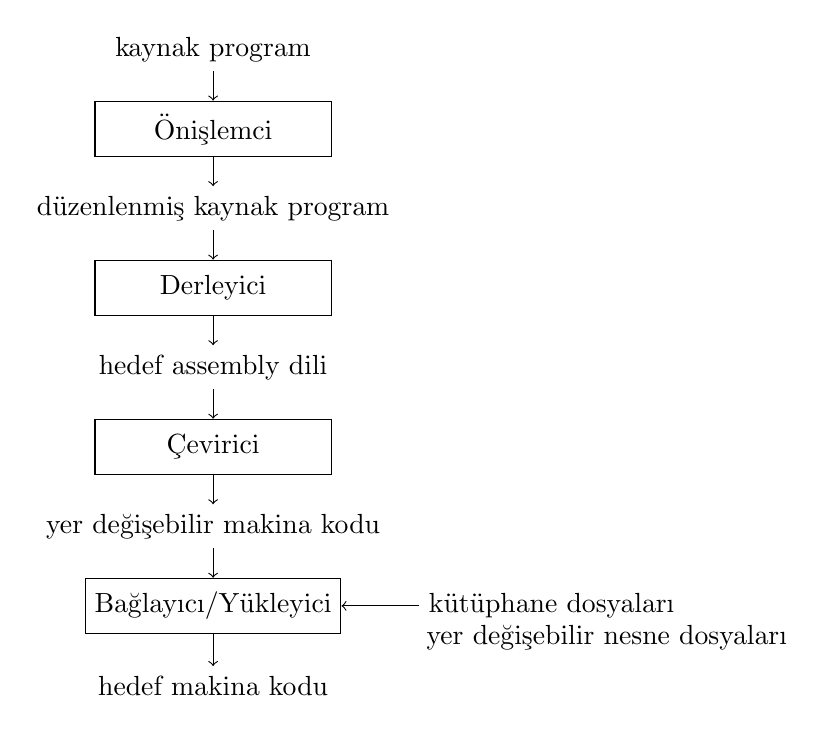
\begin{tikzpicture}[->]

\tikzstyle{rect} = [rectangle, minimum width=3cm, minimum height=0.7cm,text centered, draw=black]

\node (src_p)   {kaynak program};
\node (prep) [rect, below of=src_p, yshift=-0.01cm] {Önişlemci};   
\node (msrc_p) [below of=prep, yshift=-0.01cm]{düzenlenmiş kaynak program};
\node (cp) [rect, below of=msrc_p, yshift=-0.01cm] {Derleyici};   
\node (tr_a) [below of=cp, yshift=-0.01cm] {hedef assembly dili};
\node (as) [rect, below of=tr_a, yshift=-0.01cm]{Çevirici};   
\node (rl)  [below of=as, yshift=-0.01cm]{yer değişebilir makina kodu};
\node (ln) [rect, below of=rl, yshift=-0.01cm] {Bağlayıcı/Yükleyici};  
\node (lib) [left of=ln, xshift=6cm, yshift = -0.4cm] {yer değişebilir nesne dosyaları};
\node (lib) [left of=ln, xshift=5.3cm] {kütüphane dosyaları};
\node (out) [below of=ln, yshift=-0.01cm] {hedef makina kodu};

\draw [black](src_p) -- (prep);  
\draw [black](prep) -- (msrc_p);  
\draw [black](msrc_p) -- (cp);  
\draw [black](cp) -- (tr_a);  
\draw [black](tr_a) -- (as);  
\draw [black](as) -- (rl); 
\draw [black](rl) -- (ln);
\draw [black](ln) -- (out);
\draw [black](lib) -- (ln);   

\end{tikzpicture}

Şekil 1.5: Bir dil-işleme sistemi
\end{center}

\markboth{BÖLÜM 1. GİRİŞ}{1.2. BİR DERLEYİCİNİN YAPISI}
\section{Bir Derleyicinin Yapısı}

Bu noktaya kadar bir derleyiciye kaynak kodu, aynı semantik ile başka bir hedef programa eşleyen bir kutucuk olarak baktık. Eğer bu kutuyu biraz aralarsak aslında bu eşleme işleminin iki kısımdan oluştuğunu görürüz: analiz ve sentez.

\textit{Analiz} kısmı kaynak kodu bileşenlerine ayırır ve bu parçalar üzerinde bir sentaks yapısı uygular. Ardından bu yapıyı, kaynak kodun bir ara temsilini oluşturmak için kullanır. Eğer analiz kısmı bu aşamada sözdizimisel olarak yanlış kullanılmış veya semantik olarak belirsiz bir durum bulursa kullanıcıya, gerekli aksiyonları alması için bilgilendirici mesajlar yollamalıdır. Analiz kısmı ayrıca kaynak kod hakkında da bilgi toplar ve bunu \textit{sembol tablosu} denen bir veri yapısına kaydeder, ardından ara temsili ile beraber sentez kısmına iletir.

\setcounter{footnote}{0}
\textit{Sentez} kısmı, istelilen programı ara program temsilinden ve sembol tablosundaki bilgilerden inşa eder. Derleyicinin analiz kısmı genellikle \textit{ön uç}\footnote{(İng.) Front end. (Ç.N.)} , sentez kısmı içine \textit{arka uç}\footnote{(İng.) Back end. (Ç.N.)}  olarak isimlendirilir.

Derleme prosesini detaylı bir şekilde incelersek, kaynak programın her bir temsilini bir diğerine çeviren bir aşamalar dizisi görürüz. Tipik bir derleyicinin aşamalar halinde ayrılmış gösterimi Şekil 1.6'da gösterilmiştir. Pratikte birkaç aşama birlikte gruplanmış olabilir ve gruplandırılmış aşamalar arasındaki ara temsillerin açıkça belirtilmesine gerek yoktur. Tüm kaynak program hakkındaki bilgileri barındıran sembol tablosu derleyicinin tüm aşamaları tarafından kullanılır.

\begin{center}
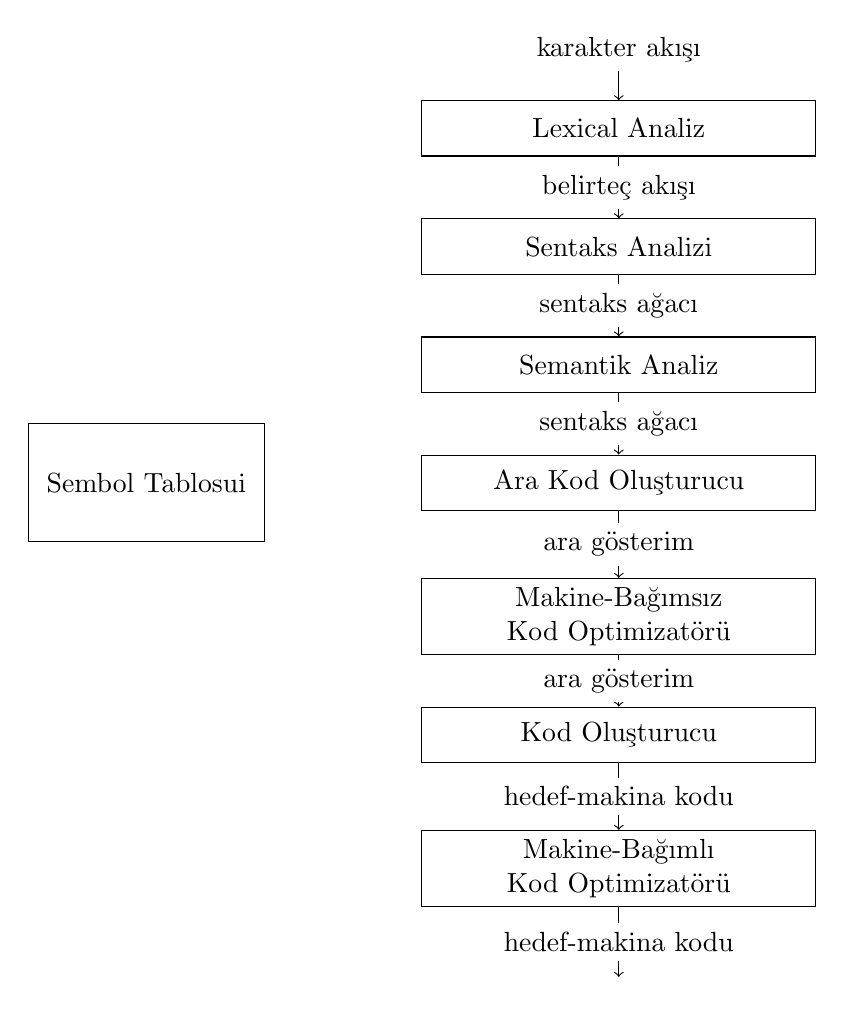
\begin{tikzpicture}[->]
\tikzstyle{rect} = [rectangle, minimum width=5cm, minimum height=0.7cm,text centered, draw=black]
\node (c_str)   {karakter akışı};
\node (lex) [rect, below of=c_str, yshift=-0.01cm] {Lexical Analiz};   
\node (syn) [rect, below of=lex, yshift=-0.5cm] {Sentaks Analizi};   
\node (smn) [rect, below of=syn, yshift=-0.5cm]{Semantik Analiz};   
\node (icode) [rect, below of=smn, yshift=-0.5cm] {Ara Kod Oluşturucu};  
\node (opt) [rect, below of=icode, yshift=-0.7cm,text width=3cm] {Makine-Bağımsız Kod Optimizatörü};  
\node (gen) [rect, below of=opt, yshift=-0.5cm] {Kod Oluşturucu};  
\node (dep_op) [rect, below of=gen, yshift=-0.7cm, text width=3cm,align=center] {Makine-Bağımlı\\Kod Optimizatörü};  
\node (dummy)  [below of=dep_op, yshift=-0.5cm] {};
\node (symbl) [rect, left of=icode, xshift=-5cm, minimum height=1.5cm, minimum width=3cm] {Sembol Tablosui};  

\draw [black](c_str) -- (lex);  
\draw [black](lex) -- node[midway,fill=white] {belirteç akışı} (syn);  
\draw [black](syn) -- node[midway,fill=white] {sentaks ağacı} (smn);  
\draw [black](smn) -- node[midway,fill=white] {sentaks ağacı} (icode);  
\draw [black](icode) -- node[midway,fill=white] {ara gösterim} (opt);  
\draw [black](opt) -- node[midway,fill=white] {ara gösterim} (gen);  
\draw [black](gen) -- node[midway,fill=white] {hedef-makina kodu} (dep_op); 
\draw [black](dep_op) -- node[midway,fill=white] {hedef-makina kodu} (dummy); 

\end{tikzpicture}

Şekil 1.6: Bir derleyicinin aşamaları
\end{center}

Bazı derleyiciler ön uç ile arka uç arasında bir makina-bağımsız kod optimizatörü barındırırlar. Bu optimizasyon, aksi takdirde optimize edilmemiş bir ara form'u çevirecek olmasından dolayı, arka ucun daha iyi bir hedef program oluşturması için kullanılan, ara form üzerindeki transformasyonları gerçekleştiren bir aşamadır. Optimizasyon opsiyonel olduğundan dolayı, Şekil 1.6'da gösterilen bir veya her iki optimizasyon aşaması bazı durumlarda orada olmayabilir.

\subsection{Lexical Analiz [10hr (until here)]}

\setcounter{footnote}{0}

Bir derleyicinin ilk aşaması \textit{lexical analiz} ya da \textit{tarama} olarak adlandırılır. Lexical analizör kaynak programı oluşturan karakter akışını okur ve onları \textit{sözcükbirim\footnote{(İng.) Lexeme. (Ç.N.)}} denilen mantıklı gruplara ayırır. Her bir sözcük birim için lexical analizör kendinden sonraki sentaks analizi aşaması için çıktı olarak aşağıda görülen formda bir belirteç\footnote{(İng.) Token. (Ç.N.) Bir derleyici için, bir veri dizisindeki en küçük mantıklı bilgi formu.} oluşturur.

{\centering {\large $\langle$\textit{belirteç-adı, bağlı-değer}$\rangle$\par}}


Belirteç'in içindeki ilk komponent olan \textit{belirteç-adı,} sentaks analizi boyunca kullanılan soyut bir semboldür, ikinci komponent \textit{bağlı-değer} ise bu belirteç için sembol tablosundaki bir girdiyi gösterir. Sembol-tablosu'ndaki bilgi girdileri, semantik analiz ve koş oluşturmak için gereklidir.

Örneğin, atama durumunu içeren bir kaynak programı düşünün

\begin{equation}
 		\text{konum = baslangic + oran * 60}
\end{equation}

Bu atamadaki karakterler aşağıda gösterilen sözcükbirim'lere gruplanabilir ve sentaks analizine geçirilmek üzere belirteçler oluşturulabilir:

\begin{enumerate}

  \item {\fontfamily{ttfamily}\selectfont konum }, $\langle$\textbf{id}, 1$\rangle$ şeklinde yazılabilecek bir sözcükbirimdir. \textbf{id} burada kimlik yerine geçen soyut bir semboldür, 1 ise, {\fontfamily{ttfamily}\selectfont konum }'un sembol-tablosu'ndaki girdisini gösterir. Bir kimlik için sembol-tablosu girdisi, bu kimlik için isim ve tip gibi bilgileri tutar.
  
  \item Atama sembolü, $\langle$=$\rangle$ şeklinde yazılabilinecek bir sözcükbirim'dir. Belirteç'in herhangi bir bağlı-değer'i olmadığı için ikinci komponenti çıkardık. Belirteç-adı için \textbf{atama} gibi herhangi bir soyut sembol de kullanabilirdik, fakat simgelemde kolaylık olması açısından, soyut sembol için direkt olarak sözcükbirim'in kendisini seçtik.
  
   \item {\fontfamily{ttfamily}\selectfont baslangic}, $\langle$\textbf{id}, 2$\rangle$ gibi bir belirteçle yazılabilecek bir sözcükbirim'dir. 2, sembol-tablosu'ndaki {\fontfamily{ttfamily}\selectfont baslangic} girdisini gösterir.
   
   \item +, $\langle$+$\rangle$ belirteci olarak yazılabilicek bir sözcükbirim'dir.
   
   \item {\fontfamily{ttfamily}\selectfont oran}, $\langle$\textbf{id}, 3$\rangle$ gibi bir belirteçle yazılabilecek bir sözcükbirim'dir. 3, sembol-tablosu'ndaki {\fontfamily{ttfamily}\selectfont oran} girdisini gösterir.
   
   \item *, $\langle$*$\rangle$ belirteci olarak yazılabilicek bir sözcükbirim'dir.
   
   \renewcommand{\thefootnote}{\arabic{footnote}}
   \setcounter{footnote}{0}
   
   \item 60, $\langle$60$\rangle$ belirteci olarak yazılabilicek bir sözcükbirim'dir.\footnote{Teknik olarak, 60 sözcükbirim'i için, $\langle$\textbf{id}, 4$\rangle$ şeklinde bir token yapmamız ve 4'ün sembol tablosunda 60 tamsayısını göstermesi gerekir, fakat sayı belirteçleri konusunu Bölüm 2'ye kadar ertelememiz gerekiyor. Bölüm 3'te ise lexical analiz teknikleri işlenecek} 
   
   \renewcommand{\thefootnote}{\fnsymbol{footnote}}
    
\end{enumerate} 

Sözcükbirimleri arasındaki boşluklar lexical analizör tarafından çıkarılacaktır.

Şekil 1.7, lexical analiz'den sonra, belirteç dizisi şeklinde, (1.1)'deki atama ifadesi gösterilir.
\newsavebox\id
\newsavebox\eq
\newsavebox\pl
\newsavebox\ml
\newsavebox\nm
\savebox\nm{\lstinline{60}}
\savebox\ml{\lstinline{*}}
\savebox\pl{\lstinline{+}}
\savebox\eq{\lstinline{=}}
\savebox\id{\lstinline{id}}

\begin{center}
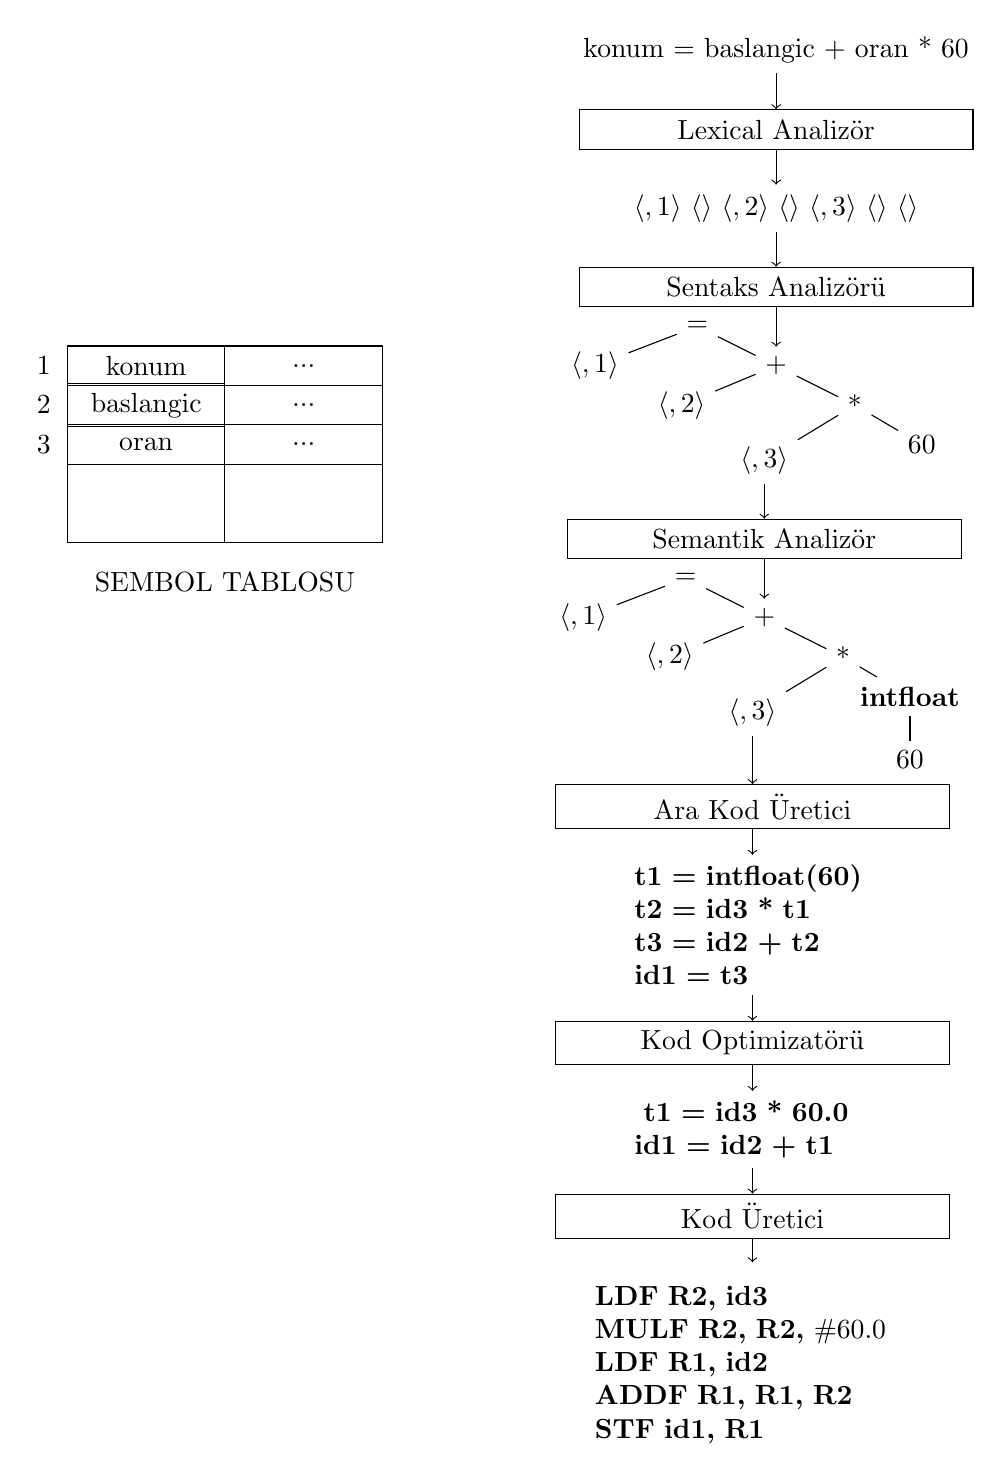
\begin{tikzpicture}[->]
\tikzstyle{rect} = [rectangle, minimum width=5cm, minimum height=0.5cm,text centered, draw=black]

\node (code)   {konum = baslangic + oran * 60};
\node (lex) [rect, below of=code, yshift=-0.01cm] {Lexical Analizör};   
\node (token)   [below of=lex, yshift=0cm]{ $\langle\usebox{\id},1\rangle$ $\langle\usebox{\eq}\rangle$ $\langle\usebox{\id},2\rangle$ $\langle\usebox{\pl}\rangle$ $\langle\usebox{\id},3\rangle$ $\langle\usebox{\ml}\rangle$ $\langle\usebox{\nm}\rangle$};

\node (syn) [rect, below of=token, yshift=0cm] {Sentaks Analizörü};   


\node (eq) [below of=syn, yshift=0.5cm, xshift=-1cm]{=};   
\node (sum) [below of=eq, yshift=0.5cm, xshift=1cm]{+};   
\node (tok1) [left of=sum, yshift=0cm,xshift=-1.3cm]{$\langle\usebox{\id},1\rangle$};  
\node (mlt) [below of=sum, yshift=0.5cm, xshift=1cm]{*};   
\node (tok2) [left of=mlt, yshift=0cm,xshift=-1.2cm]{$\langle\usebox{\id},2\rangle$};  
\node (sixty) [below of =mlt, xshift=0.85cm, yshift=0.5cm]{60};   
\node (tok3) [left of=sixty, xshift=-1cm, yshift=-0.2cm]{$\langle\usebox{\id},3\rangle$};   
\draw [black, -](mlt) -- (sixty);  
\draw [black, -](mlt) -- (tok3);  
\draw [black, -](sum) -- (mlt);  
\draw [black, -](sum) -- (tok2);  
\draw [black, -](eq) -- (sum);  
\draw [black, -](eq) -- (tok1);  

\node (smn) [rect, below of=tok3, yshift=0cm] {Semantik Analizör};   

\node (eq2) [below of=smn, yshift=0.5cm, xshift=-1cm]{=};   
\node (sum2) [below of=eq2, yshift=0.5cm, xshift=1cm]{+};   
\node (tok12) [left of=sum2, yshift=0cm,xshift=-1.3cm]{$\langle\usebox{\id},1\rangle$};  
\node (mlt2) [below of=sum2, yshift=0.5cm, xshift=1cm]{*};   
\node (tok22) [left of=mlt2, yshift=0cm,xshift=-1.2cm]{$\langle\usebox{\id},2\rangle$};  
\node (int) [below of =mlt2, xshift=0.85cm, yshift=0.5cm]{\textbf{intfloat}};   
\node (sixty2) [below of =int, xshift=0cm, yshift=0.2cm]{60};   
\node (tok32) [left of=int, xshift=-1cm, yshift=-0.2cm]{$\langle\usebox{\id},3\rangle$};   
\draw [black, -](mlt2) -- (int);  
\draw [black, -](mlt2) -- (tok32);  
\draw [black, -](sum2) -- (mlt2);  
\draw [black, -](sum2) -- (tok22);  
\draw [black, -](eq2) -- (sum2);  
\draw [black, -](eq2) -- (tok12);  
\draw [black, -](int) -- (sixty2);  

\node (mdt) [rect, below of=tok32, yshift=-0.2cm] {Ara Kod Üretici};   
\node (cline) [ below of=mdt, yshift=-0.5cm, text width = 3cm] {
	\textbf{t1 = intfloat(60) 
		  t2 = id3 * t1\\ 
		  t3 = id2 + t2\\
		  id1 = t3
		  }
	
	};   
	
\node (opt) [rect, below of=cline, yshift=-0.5cm] {Kod Optimizatörü};   

\node (cline2) [ below of=opt, yshift=-0.1cm, text width = 3cm] {
	\textbf{
		  t1 = id3 * 60.0
		  id1 = id2 + t1
		  }
	
	};   
	
\node (gnr) [rect, below of=cline2, yshift=-0.1cm] {Kod Üretici};   

\node (assm) [ below of=gnr, yshift=-0.8cm, text width = 4cm] {

	\textbf{LDF R2, id3\\
		 MULF R2, R2, $\#60.0$\\
		 LDF R1, id2\\
		 ADDF R1, R1, R2\\
		 STF id1, R1
		  }
	
	};   
	
	\node (r1_val) [rect, left of=syn, xshift=-5cm, yshift=-1cm, minimum width=2cm] {...}; 
	\node (r1) [rect, left of=r1_val, xshift=-1cm, minimum width=2cm] {konum};   
	\node (r2_val) [rect, below of=r1_val, yshift=0.5cm, minimum width=2cm] {...}; 
	\node (r2) [rect, left of=r2_val, xshift=-1cm, minimum width=2cm] {baslangic};   
	\node (r3_val) [rect, below of=r2_val, yshift=0.5cm, minimum width=2cm] {...}; 
	\node (r3) [rect, left of=r3_val, xshift=-1cm, minimum width=2cm] {oran};   
	\node (r3_val) [rect, below of=r3_val, yshift=0.25cm, minimum width=2cm,minimum height=1cm] {}; 
	\node (r4) [rect, below of=r3, yshift=0.25cm, minimum width=2cm, minimum height=1cm] {};   
	
	\node (n1)[left of = r1, xshift=-0.3cm]   {1};
	\node (n2)[left of = r2, xshift=-0.3cm]    {2};
	\node (n3)[left of = r3, xshift=-0.3cm]    {3};
	\node (s)[below of = r4, xshift=1cm]    {SEMBOL TABLOSU};
	
\draw [black](code) -- (lex);  
\draw [black](lex) -- (token);  
\draw [black](token) -- (syn);  
\draw [black](syn) -- (sum);  
\draw [black](tok3) -- (smn);  
\draw [black](smn) -- (sum2);
\draw [black](tok32) -- (mdt);  
\draw [black](mdt) -- (cline);  
\draw [black](cline) -- (opt);  
\draw [black](opt) -- (cline2);  
\draw [black](cline2) -- (gnr);  
\draw [black](gnr) -- (assm);  

\end{tikzpicture}

Şekil 1.7: Bir atama işleminin çevrilmesi
\end{center}


\begin{equation}
 		\text{ $\langle\usebox{\id},1\rangle$ $\langle\usebox{\eq}\rangle$ $\langle\usebox{\id},2\rangle$ $\langle\usebox{\pl}\rangle$ $\langle\usebox{\id},3\rangle$ $\langle\usebox{\ml}\rangle$ $\langle\usebox{\nm}\rangle$}
\end{equation}

Bu gösterimde belirteç adları, =, + ve *, atama, toplama ve çıkarma işlemleri için soyut sembollerdir.


\subsection{Sentaks Analizi [52min]}
Derleyicinin ikinci aşaması sentaks analizi'dir\footnote{Bazen \textit{Syntax Analysis} bazen de \textit{Parsing} olarak gösterilir (Ç.N.)}. Sentaks analizi, lexical analizör tarafından oluşturulan belirteçlerin ilk komponentlerini, bu belirteç akışının gramatik yapısını tasvir eden ağaç yapısı türünde bir ara kod gösterimi olşturmak için kullanır. Sentaks ağacı tipik bir gösterimdir; her iç düğüm bir operasyonu, ve bu düğümlerin çocuk düğümleri ise operasyonun argümanlarını temsil eder. (1.2)'deki belirteç akışı'nın sentaks ağacı Şekil 1.7'de sentaktik analizör'ün çıktısı olarak gösterilmiştir.  Bu ağaç, atamadaki operasyonların çalıştırılma sırasını gösterir.
\begin{lstlisting}
 	     konum = baslangic + oran * 60        
\end{lstlisting}
Ağaç, * ile etiketlenmiş, $\langle$\textbf{id}, 3$\rangle$'ün sol çocuk, 60 tamsayısının da sağ çocuk düğümü olarak tanımlandığı bir iç düğüme sahiptir. $\langle$\textbf{id}, 3$\rangle$, \textbf{oran} tanımlayıcısını temsil eder. * ile etiketlenmiş düğüm, ilk önce \textbf{oran}'ın değeri ile 60'ı çarpmamız gerektiğini belirgin bir şekilde gösterir. + ile işaretlenmiş düğüm bu çarpım değerini \textbf{baslangic}'ın değeri ile toplamamız gerektiğini belirtir. = şeklinde etiketlenmiş, ağacın kökü olan düğüm, bu toplamın sonucunu \textbf{konum} belirtecinin olduğu lokasyona kaydetmemiz gerektiğini gösterir. Bu operasyonların sırası, geleneksel aritmetik ile tutarlıdır; çarpımın, toplamadan daha yüksek önceliği vardır, dolayısıyla çarpma operasyonu, toplamadan önce gerçekleştirilmelidir.

Bundan sonra gelen derleyici aşamaları gramatik yapıyı, hedef programı üretmek için kaynak programın analizinde yardımcı olarak kullanırlar. Bölüm 4'te bağlam-duyarsız gramerleri programlama dillerinin yapısını belirtmek için kullanacağız ve belirli sınıf ve gramerlerden verimli sentaks analizörleri'ni otomatik olarak oluşturacak algoritmaları tartışacağız. Bölüm 2 ve 5'te sentaks-yönelimli tanımlamaların, programlama dili yapılarını çevirmede yardımcı olabileceğini göreceğiz.

\subsection{Semantik Analiz [34min]}
\textit{Semantik analizör}, kaynak programın dilin tanımlamalarına göre semantik tutarlılığını, sentaks ağacını ve sembol tablosundaki bilgileri kullanarak kontrol eder. Ayrıca ileride, ara kod üretiminde kullanılmak üzere, tip bilgilerini toplayarak bunu ya sentaks ağacında ya da sembol tablosunda saklar.

Semantik analiz'in önemli bir parçası, derleyicinin her bir operatör için, o operatörün terimlerinin uyuşup uyuşmadığını kontrol ettiği \textit{tip-kontrolü}'dür. Örneğin, birçok programlama dili bir dizinin indis değerlerinin tamsayı olmasını ister; derleyici, dizi indisi belirtmek için eğer ondalık bir sayı kullanılmışsa, bunun için bir hata raporu vermelidir.

Dil spesifikasyonları, \textit{zorlama}\footnote{(İng.) Coercion (Ç.N.)} adı verilen bazı tip çevrimlerine izin veriyor olabilir. Örneğin bir binary aritmetik operatörü bir tamsayı çiftine ya da bir ondalıklı sayı çiftine uygulanabilir. Eğer operatör bir tamsayı ve bir ondalıklı sayıya uygulanmışsa, derleyici tamsayıyı ondalıklıya, ya da ondalıklı sayıyı tamsayıya çevirebilir veya zorlayabilir.

Böyle bir zorlama Şekil 1.7'de görünür. Farz edin ki, \textbf{konum}, \textbf{baslangic} ve \textbf{oran} ondalık sayı olarak tanımlanmış ve \textbf{60} ise kendinden dolayı bir tamsayı olsun. Şekil 1.7'deki semantik analizörün içindeki tip-kontrolcüsü * operatörünün bir ondalık sayı olan \textbf{oran}, ve bir tam sayı olan \textbf{60} için uygulandığını fark edecek. Bu durumda tamsayı, bir ondalıklı sayıya çevrilebilir. Şekil 1.7'de semantik analizörün \textbf{inttofloat} için fazladan bir düğümü olduğuna dikkat edin; ki açıkça tamsayı türündeki bir argümanı ondalıklı sayıya çevirir. Tip kontrolü ve semantik analiz Bölüm 6'da tartışılacaktır.

\subsection{Ara Kod Üretimi [50min]}
Bir kaynak programı hedef programa çevirme sürecinde, derleyici çeşitli formlarda birden fazla ara kod üretebilir. Sentaks ağaçları bir ara gösterim formlarıdır; bu formlar sentaks ve semantik analizinde yaygın olarak kullanılırlar.

Kaynak programın sentaks ve semantik analizinden sonra, birçok derleyici belirgin bir düşük-seviye ya da makine-tipi bir ara gösterim oluşturur; bunu soyut bir makina için bir program olarak düşünebiliriz. Bu ara gösterimin iki önemli özelliği vardır: üretilmesinin ve kaynak makineye çevrilmesinin kolaylığı.

Bölüm 6'da, bir dizi assembly benzeri, komut barındıran (komut başına üç terim), \textit{üç-adres} denen bir ara formu inceleyeceğiz. Her terim bir register olarak davranabilir. Şekil 1.7'deki ara kod üreticinin çıktısı, üç-adres kod dizisi içerir.

%TODO ; Fix the following equation
\begin{equation*}
\text{ t1 = intfloat(60) }
\end{equation*}
\begin{equation*}
\text{ t2 = id3 * t1 }
\end{equation*}
\begin{equation}
\text{ t3 = id2 + t2 }
\end{equation}
\begin{equation*}
\text{ id1 = t3 }
\end{equation*}

Burada, üç-adres komutları için hiçbir değeri olmayan bazı noktalar bulunuyor. Öncelikle her üç-adress ataması, sağ kısmında en fazla bir operatör bulundurur. Böylece, bu komutlar işlemlerin gerçekleştirilme sıralarını doğrular; kaynak kodda (1.1) çarpma, toplamadan önce geliyor. Ardından derleyici üç-adres komutu tarafından hesaplanmış değeri tutmak için geçici bir isim üretmelidir. Son olarak, yukarıdaki ilk ve son satır'daki (1.3) gibi bazı "üç-adres komutları" üçten az terime sahiptir.

Bölüm 6'da derleyicilerde kullanılan asıl ara gösterimleri işleyeceğiz. Bölüm 5, Bölüm 6'da ifadeler, kontrol-akışı ve prosedür çağrıları gibi tipik programlama dili yapıları için tip-kontrol ve ara-kod üretimi üzerinde uygulanmak üzere sentaks-yönelimli çevrim tekniklerini tanıtır.

